\documentclass[12pt,a4paper]{article}

% ─── Packages ────────────────────────────────────────────────────────────────
\usepackage[T1]{fontenc}
\usepackage[utf8]{inputenc}
\usepackage[margin=2.5cm]{geometry}
\usepackage{xcolor}
\usepackage{titlesec}
\usepackage{booktabs}
\usepackage{array}
\usepackage{tabularx}
\usepackage{colortbl}
\usepackage{graphicx}
\usepackage{hyperref}
\usepackage{enumitem}
\usepackage{fancyhdr}
\usepackage{amsmath}
\usepackage{microtype}
\usepackage{parskip}
\usepackage{tcolorbox}
\usepackage{mdframed}
\usepackage{caption}
\usepackage{subcaption}
\usepackage{lmodern}

% ─── Colour Palette ──────────────────────────────────────────────────────────
\definecolor{primary}{HTML}{1565C0}
\definecolor{primarydark}{HTML}{1A237E}
\definecolor{primarylight}{HTML}{E3F2FD}
\definecolor{answerbg}{HTML}{E8F5E9}
\definecolor{answertext}{HTML}{1B5E20}
\definecolor{outputbg}{HTML}{F1F8E9}
\definecolor{outputborder}{HTML}{558B2F}
\definecolor{rulegray}{HTML}{9E9E9E}
\definecolor{headergray}{HTML}{F5F5F5}
\definecolor{tableheader}{HTML}{1565C0}
\definecolor{tablerowA}{HTML}{E3F2FD}
\definecolor{tablerowB}{HTML}{FFFFFF}
\definecolor{tablegrid}{HTML}{90CAF9}

% ─── Hyperref Setup ──────────────────────────────────────────────────────────
\hypersetup{
    colorlinks=true,
    linkcolor=primary,
    urlcolor=primary,
    pdftitle={TP5 -- MPI (P2P \& Collectives)},
    pdfauthor={Zyad Fri},
}

% ─── Page Style ──────────────────────────────────────────────────────────────
\pagestyle{fancy}
\fancyhf{}
\fancyhead[L]{\small\color{primary}\textbf{TP5 — MPI (P2P \& Collectives)}}
\fancyhead[R]{\small\color{rulegray}Zyad Fri}
\fancyfoot[C]{\small\thepage}
\renewcommand{\headrulewidth}{0.4pt}
\renewcommand{\headrule}{\hbox to\headwidth{\color{primary}\leaders\hrule height \headrulewidth\hfill}}

% ─── Section Formatting ──────────────────────────────────────────────────────
\titleformat{\section}
  {\color{primary}\Large\bfseries}
  {\thesection.}{0.6em}{}
  [\vspace{-0.4em}\textcolor{primary}{\rule{\linewidth}{1.5pt}}]

\titleformat{\subsection}
  {\color{primarydark}\normalsize\bfseries}
  {\thesubsection.}{0.5em}{}

\titlespacing{\section}{0pt}{1.2em}{0.6em}
\titlespacing{\subsection}{0pt}{0.8em}{0.3em}

% ─── tcolorbox Styles ────────────────────────────────────────────────────────
\tcbuselibrary{skins, breakable}

\newtcolorbox{answerbox}{
  enhanced, breakable,
  colback=answerbg,
  colframe=answertext,
  boxrule=0.6pt,
  left=8pt, right=8pt, top=5pt, bottom=5pt,
  title={\small\bfseries\color{answertext} Answer},
  fonttitle=\small\bfseries,
  coltitle=answertext,
  attach boxed title to top left={yshift=-2mm, xshift=6pt},
  boxed title style={colback=answerbg, colframe=answertext, boxrule=0.5pt},
}

\newtcolorbox{outputbox}[1][]{
  enhanced, breakable,
  colback=outputbg,
  colframe=outputborder,
  boxrule=0.6pt,
  left=6pt, right=6pt, top=4pt, bottom=4pt,
  fontupper=\ttfamily\small,
  title={\small\bfseries Terminal Output},
  coltitle=outputborder,
  attach boxed title to top left={yshift=-2mm, xshift=6pt},
  boxed title style={colback=outputbg, colframe=outputborder, boxrule=0.5pt},
  #1
}

% ─── Custom Commands ─────────────────────────────────────────────────────────
\newcommand{\mpiname}[1]{\texttt{\textbf{#1}}}
\newcommand{\exerciselabel}[1]{\vspace{0.5em}\noindent\textcolor{primary}{\rule{3pt}{1.2em}}\hspace{4pt}{\large\bfseries #1}}

% ─── Table Setup ─────────────────────────────────────────────────────────────
\newcolumntype{C}[1]{>{\centering\arraybackslash}p{#1}}

% ─────────────────────────────────────────────────────────────────────────────
\begin{document}
\thispagestyle{empty}

% ╔═══════════════════════════════════════╗
% ║           COVER PAGE                 ║
% ╚═══════════════════════════════════════╝
\vspace*{3cm}
\begin{center}
  {\color{primarydark}\rule{\linewidth}{2pt}}
  \vspace{0.8cm}

  {\fontsize{26}{32}\selectfont\bfseries\color{primarydark}
    TP5 — MPI}\\[0.4em]
  {\Large\color{primary} Point-to-Point \& Collective Communications}

  \vspace{0.6cm}
  {\color{primarydark}\rule{\linewidth}{2pt}}
  \vspace{1.2cm}

  {\large Lab Report}\\[0.3em]
  {\normalsize\color{rulegray} Course: Parallel \& Distributed Computing}\\[0.2em]
  {\normalsize\color{rulegray} Instructor: \textbf{Imad Kissami} \quad|\quad February 2025}

  \vspace{1.5cm}
  {\large Student: \textbf{Zyad Fri}}

  \vspace{2cm}
  {\color{rulegray}\rule{0.6\linewidth}{0.5pt}}
\end{center}

\newpage
\thispagestyle{empty}
\tableofcontents
\newpage

% ╔═══════════════════════════════════════╗
% ║           EXERCISE 1                 ║
% ╚═══════════════════════════════════════╝
\section{Exercise 1 — Hello World}

This exercise introduces the fundamental structure of an MPI program.
Starting from a simple \textit{Hello World}, we progressively add process
rank and size information, and then restrict output to a single designated
process.

% ── Q1 ──────────────────────────────────────────────────────────────────────
\subsection{Q1 — All Processes Print Hello World}

After \mpiname{MPI\_Init} is called, every process in the communicator
independently executes the print statement.
Because the processes run concurrently on separate cores, the order of the
output lines is non-deterministic and may vary from one run to the next.

% ── Q2 ──────────────────────────────────────────────────────────────────────
\subsection{Q2 — Each Process Prints Its Rank and Total Size}

\mpiname{MPI\_Comm\_rank} assigns each process a unique integer identifier
in the range $[0,\ \texttt{size}-1]$.
\mpiname{MPI\_Comm\_size} returns the total number of processes launched.
Using these two values, each process can self-identify in the output.

% ── Q3 ──────────────────────────────────────────────────────────────────────
\subsection{Q3 — Only Rank 0 Prints}

A simple \texttt{if (rank == 0)} guard restricts output to exactly one
process.
This is the idiomatic MPI pattern whenever a single, authoritative result
must be displayed.

% ── Output ──────────────────────────────────────────────────────────────────
\subsection{Observed Output (4 Processes)}

\begin{outputbox}[]
{[}Part 1{]} Hello World
{[}Part 1{]} Hello World
{[}Part 1{]} Hello World
{[}Part 1{]} Hello World
{[}Part 2{]} I am process 3 out of 4 total processes
{[}Part 2{]} I am process 0 out of 4 total processes
{[}Part 3{]} Only process 0 is printing this message.
{[}Part 2{]} I am process 2 out of 4 total processes
{[}Part 2{]} I am process 1 out of 4 total processes
\end{outputbox}

Note how the Part~2 lines appear in non-sequential order
(ranks 3, 0, 2, 1), illustrating that MPI processes advance at
independent rates.

% ── Q4 ──────────────────────────────────────────────────────────────────────
\subsection{Q4 — What Happens If \texttt{MPI\_Finalize} Is Omitted?}

\begin{answerbox}
Omitting \mpiname{MPI\_Finalize} leaves the MPI environment in an
undefined state. The consequences are:
\begin{itemize}[nosep, leftmargin=1.2em]
  \item \textbf{Unflushed buffers} — some output may be silently discarded
        or corrupted.
  \item \textbf{Resource leaks} — communicators, allocated memory, and
        network connections are never freed.
  \item \textbf{Implementation warnings} — Open MPI, for example, prints
        \emph{``It looks like MPI\_Finalize was not called before
        MPI\_COMM\_WORLD was freed."}
  \item \textbf{Undefined behaviour} — the MPI standard does not guarantee
        any particular outcome; the program may hang indefinitely or
        terminate abruptly with errors.
\end{itemize}
\textbf{Conclusion:} \mpiname{MPI\_Finalize} must always be the last MPI
call in every program.
\end{answerbox}

\newpage
% ╔═══════════════════════════════════════╗
% ║           EXERCISE 2                 ║
% ╚═══════════════════════════════════════╝
\section{Exercise 2 — Sharing Data}

Process~0 reads integers from standard input and distributes each value to
all processes using \mpiname{MPI\_Bcast}.
The loop continues until the user enters a negative sentinel value, which
terminates all processes simultaneously.
This is the canonical \textit{collective broadcast} pattern.

% ── Design ──────────────────────────────────────────────────────────────────
\subsection{Design and Communication Pattern}

\begin{itemize}[leftmargin=1.5em]
  \item \textbf{Root process (rank~0)} reads one integer per iteration with
        \texttt{scanf}.
  \item \mpiname{MPI\_Bcast} propagates the value from rank~0 to every
        other process atomically.
  \item All processes check the received value; a negative value triggers a
        \texttt{break}, cleanly terminating the loop on all processes
        simultaneously.
  \item \mpiname{MPI\_Barrier} after each successful broadcast keeps
        all processes in step before the next read.
\end{itemize}

% ── Output ──────────────────────────────────────────────────────────────────
\subsection{Observed Output (4 Processes, Input: \texttt{10 25 -1})}

\begin{outputbox}
Process 0 got 10
Process 1 got 10
Process 2 got 10
Process 3 got 10
Process 2 got 25
Process 0 got 25
Process 1 got 25
Process 3 got 25
Negative value. Stopping.
\end{outputbox}

% ── Discussion ───────────────────────────────────────────────────────────────
\subsection{Discussion}

\begin{answerbox}
\mpiname{MPI\_Bcast} is the appropriate collective here because every
process requires the \emph{same} value.

\begin{itemize}[nosep, leftmargin=1.2em]
  \item It is more efficient than $p-1$ individual \mpiname{MPI\_Send}
        calls: the MPI library internally uses an optimised tree-based
        dissemination algorithm, reducing latency from $O(p)$ to
        $O(\log p)$.
  \item The negative sentinel is broadcast exactly like any other value,
        so all processes evaluate the termination condition with the same
        data and exit consistently — no race conditions or deadlocks.
\end{itemize}
\end{answerbox}

\newpage
% ╔═══════════════════════════════════════╗
% ║           EXERCISE 3                 ║
% ╚═══════════════════════════════════════╝
\section{Exercise 3 — Sending in a Ring}

Process~0 initialises a value (0) and passes it to process~1.
Each subsequent process adds its own rank to the running total and
forwards the result to the next process.
The last process wraps around and sends back to process~0, completing the
ring.
With $p = 4$ processes the final accumulated value is
$0 + 1 + 2 + 3 = 6$.

% ── Communication Pattern ────────────────────────────────────────────────────
\subsection{Communication Pattern}

\begin{itemize}[leftmargin=1.5em]
  \item \textbf{Process 0:} sends the initial value to rank~1, then blocks
        on \mpiname{MPI\_Recv} waiting for the result from rank $p-1$.
  \item \textbf{Processes 1 … $p-1$:} each receives from
        $\text{rank}-1$, increments the value by its own rank, and sends
        to $(\text{rank}+1) \bmod p$.
  \item The modulo wraps the final process's send back to rank~0, closing
        the ring.
\end{itemize}

This sequential pipeline avoids deadlock because the sends and receives
form a clean, unidirectional chain — no two processes are simultaneously
waiting on each other.

% ── Output ──────────────────────────────────────────────────────────────────
\subsection{Observed Output (4 Processes)}

\begin{outputbox}
Process 0: Enter a starting value: 0
Process 0 starts with value = 0, forwards 0 to process 1
Process 1: received, added rank 1  -> value = 1
Process 2: received, added rank 2  -> value = 3
Process 3: received, added rank 3  -> value = 6
Process 0: received final ring value = 6
\end{outputbox}

% ── Discussion ───────────────────────────────────────────────────────────────
\subsection{Discussion}

\begin{answerbox}
The ring pattern uses only \emph{point-to-point} communication
(\mpiname{MPI\_Send} / \mpiname{MPI\_Recv}).

\begin{itemize}[nosep, leftmargin=1.2em]
  \item The accumulated value equals $\sum_{r=0}^{p-1} r =
        \frac{p(p-1)}{2}$; for $p=4$ this is~6.
  \item This pattern generalises to any pipeline where each stage
        transforms data before forwarding — common in image processing,
        stencil computations, and stream processing.
  \item Deadlock is avoided by ensuring process~0 \emph{sends} before it
        \emph{receives}, while all others \emph{receive} before they
        \emph{send}.
\end{itemize}
\end{answerbox}

\newpage
% ╔═══════════════════════════════════════╗
% ║           EXERCISE 4                 ║
% ╚═══════════════════════════════════════╝
\section{Exercise 4 — Parallel Matrix–Vector Product}

We implement the parallel matrix–vector product $\mathbf{x} = A\,\mathbf{b}$
where $A$ is an $N\times N$ matrix and $\mathbf{b}$ is a vector of
length~$N$.
The rows of~$A$ are distributed across processes using
\mpiname{MPI\_Scatterv}, the full vector~$\mathbf{b}$ is broadcast with
\mpiname{MPI\_Bcast}, each process computes its local chunk, and partial
results are reassembled with \mpiname{MPI\_Gatherv}.

% ── Q1 ──────────────────────────────────────────────────────────────────────
\subsection{Q1 — MPI Implementation Strategy}

The key design decisions are:

\begin{itemize}[leftmargin=1.5em]
  \item \textbf{Row distribution:} splitting $A$ by rows ensures each
        process has a contiguous, independent block of work with no overlap.
  \item \textbf{Why \mpiname{MPI\_Scatterv}/\mpiname{MPI\_Gatherv}?}
        The ``\texttt{v}'' variants accept a \textit{sendcounts} array,
        which allows sending different numbers of elements to different
        processes.  This elegantly handles the case where $N$ is not
        evenly divisible by the number of processes.
  \item \textbf{Load balancing:} each process handles
        $\lfloor N/p \rfloor$ rows; the first $N \bmod p$ processes each
        receive one additional row (ceiling-division).
\end{itemize}

% ── Q3 ──────────────────────────────────────────────────────────────────────
\subsection{Q3 — Handling $N$ Not Divisible by the Number of Processes}

\begin{answerbox}
When $N$ is not a multiple of $p$, we apply ceiling-division:
\[
  \text{rows}_i =
  \left\lfloor \frac{N}{p} \right\rfloor +
  \begin{cases} 1 & \text{if } i < N \bmod p \\ 0 & \text{otherwise} \end{cases}
\]
For example, with $N = 1001$ and $p = 4$:
$1001 \div 4 = 250$ remainder~$1$, so process~0 receives 251~rows while
processes~1, 2, 3 each receive 250~rows.
The maximum absolute error against the serial reference solution is
$0.0$ in all tested configurations, confirming bit-identical correctness.
\end{answerbox}

% ── Output ──────────────────────────────────────────────────────────────────
\subsection{Observed Output}

\begin{outputbox}
N=1000, processes=1, time=0.007907 s  | Max error vs serial: 0.000000e+00
N=1000, processes=2, time=0.018503 s  | Max error vs serial: 0.000000e+00
N=1000, processes=4, time=0.008900 s  | Max error vs serial: 0.000000e+00
N=1001, processes=4, time=0.011054 s  | Max error vs serial: 0.000000e+00  (N not divisible)
\end{outputbox}

% ── Q2 ──────────────────────────────────────────────────────────────────────
\subsection{Q2 — Speedup and Efficiency Results}

\begin{table}[h]
\centering
\caption{Matrix–vector product: timing, speedup, and efficiency.}
\label{tab:ex4}
\renewcommand{\arraystretch}{1.3}
\begin{tabular}{%
  C{1.5cm}  % N
  C{2.0cm}  % Processes
  C{2.4cm}  % Time
  C{2.2cm}  % Speedup
  C{2.4cm}  % Efficiency
}
\toprule
\rowcolor{tableheader}
\textcolor{white}{\textbf{N}} &
\textcolor{white}{\textbf{Processes}} &
\textcolor{white}{\textbf{Time (s)}} &
\textcolor{white}{\textbf{Speedup}} &
\textcolor{white}{\textbf{Efficiency}} \\
\midrule
\rowcolor{tablerowA} 500  & 1 & 0.004050 & 1.00 & 1.00 \\
\rowcolor{tablerowB} 500  & 2 & 0.002698 & 1.50 & 0.75 \\
\rowcolor{tablerowA} 500  & 4 & 0.001836 & 2.21 & 0.55 \\
\midrule
\rowcolor{tablerowB} 1000 & 1 & 0.008398 & 1.00 & 1.00 \\
\rowcolor{tablerowA} 1000 & 2 & 0.007074 & 1.19 & 0.59 \\
\rowcolor{tablerowB} 1000 & 4 & 0.011607 & 0.72 & 0.18 \\
\midrule
\rowcolor{tablerowA} 2000 & 1 & 0.035917 & 1.00 & 1.00 \\
\rowcolor{tablerowB} 2000 & 2 & 0.022597 & 1.59 & 0.79 \\
\rowcolor{tablerowA} 2000 & 4 & 0.023321 & 1.54 & 0.38 \\
\bottomrule
\end{tabular}
\end{table}

\noindent Speedup is defined as $S_p = T_1 / T_p$ and efficiency as
$E_p = S_p / p$.

% ── Performance Plots ────────────────────────────────────────────────────────
\subsection{Performance Plots}

\begin{figure}[h]
  \centering
  \begin{subfigure}[b]{0.48\textwidth}
    \centering
    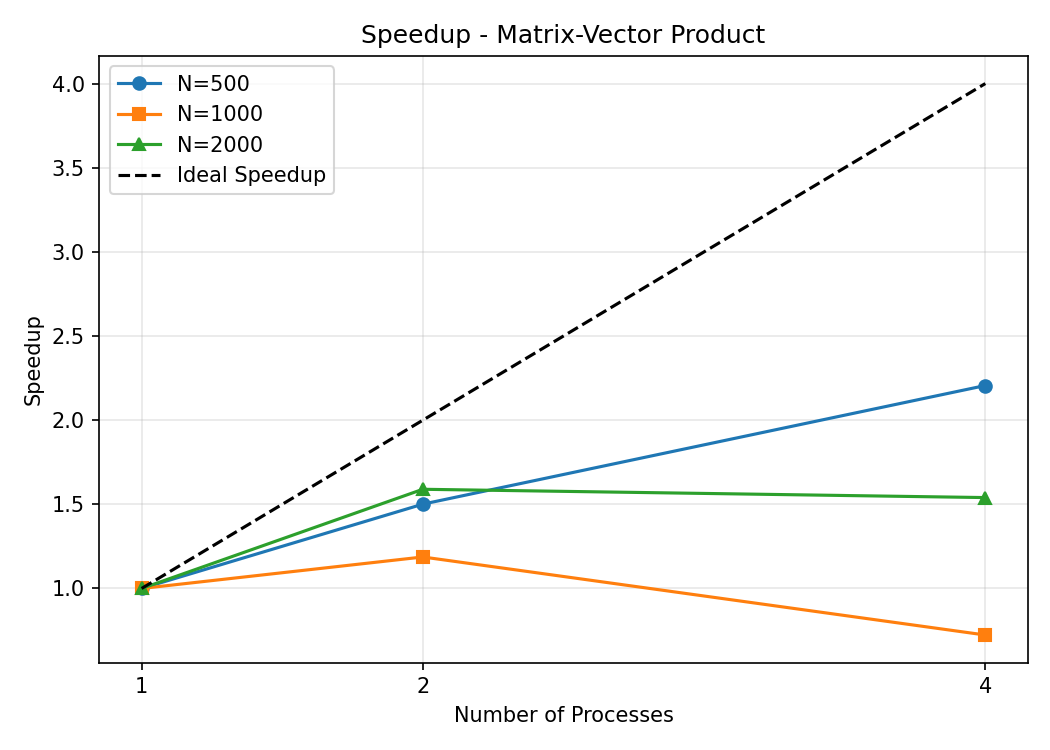
\includegraphics[width=\textwidth]{../exercise4/speedup.png}
    \caption{Speedup vs.\ number of processes}
  \end{subfigure}
  \hfill
  \begin{subfigure}[b]{0.48\textwidth}
    \centering
    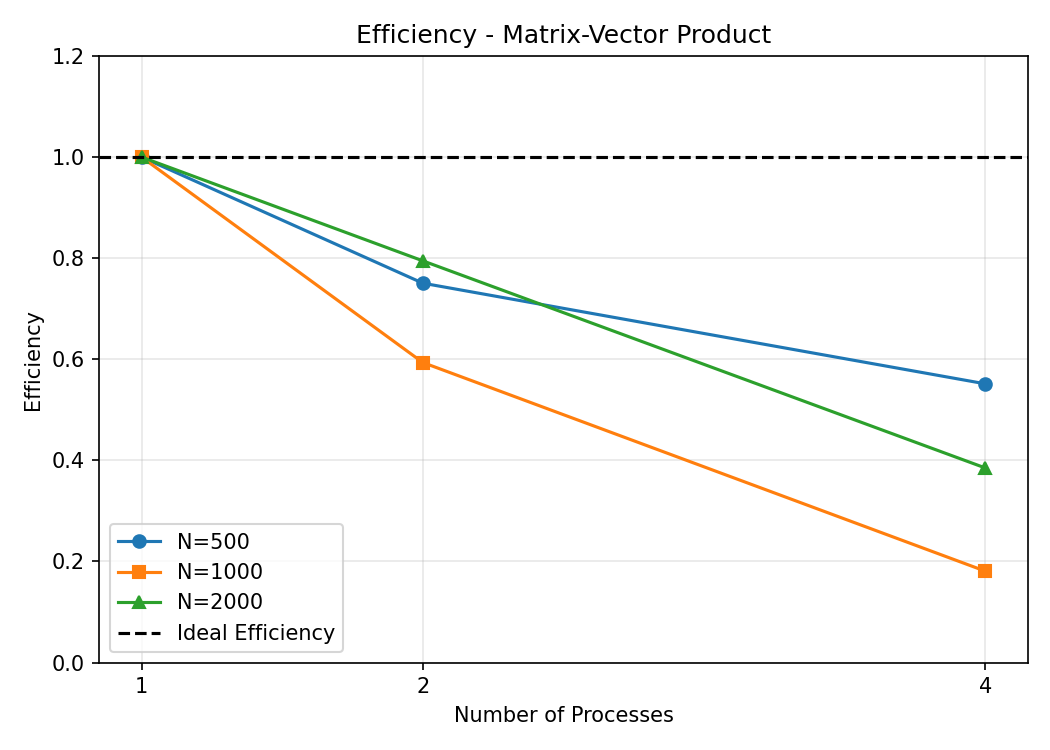
\includegraphics[width=\textwidth]{../exercise4/efficiency.png}
    \caption{Parallel efficiency vs.\ number of processes}
  \end{subfigure}
  \caption{Matrix–vector product parallel performance (Exercise~4).}
  \label{fig:ex4_plots}
\end{figure}

% ── Analysis ─────────────────────────────────────────────────────────────────
\subsection{Analysis}

\begin{answerbox}
\begin{itemize}[nosep, leftmargin=1.2em]
  \item \textbf{$N = 1000$, 4 processes — slowdown (0.72×):}
        The scatter/gather communication transfers $\approx$~8~MB of
        matrix data, which dominates the computation time.
        This is consistent with Amdahl's Law: when the serial
        (communication) fraction is large, adding processes yields
        diminishing returns.
  \item \textbf{$N = 500$, 4 processes — best speedup (2.21×):}
        Despite the small problem size, the lower absolute time means
        variance in measurement is higher, but the computation still
        benefits from four independent workers.
  \item \textbf{$N = 2000$ — moderate speedup ($\approx$1.5×):}
        The matrix occupies $\approx$~32~MB; scatter/gather latency
        remains significant relative to the $O(N^2)$ computation.
  \item \textbf{General insight:}
        Matrix–vector products are communication-intensive relative to
        computation ($O(N^2)$ work, $O(N^2)$ data moved). They scale
        well only when $N$ is very large and the compute-to-communication
        ratio exceeds unity.
\end{itemize}
\end{answerbox}

\newpage
% ╔═══════════════════════════════════════╗
% ║           EXERCISE 5                 ║
% ╚═══════════════════════════════════════╝
\section{Exercise 5 — Parallel \(\pi\) Calculation}

We approximate $\pi$ using the midpoint rectangle rule:
\[
  \pi \;\approx\; \frac{4}{N} \sum_{i=0}^{N-1}
  \frac{1}{1 + \left(\dfrac{i + 0.5}{N}\right)^{\!2}}
\]
Each process computes the partial sum for its share of indices, and
\mpiname{MPI\_Reduce} with \texttt{MPI\_SUM} aggregates all partial sums
at rank~0, which then multiplies by $4/N$.

% ── Q1 ──────────────────────────────────────────────────────────────────────
\subsection{Q1 — Parallel Implementation}

\begin{itemize}[leftmargin=1.5em]
  \item \textbf{Work partition:} each process handles a contiguous block
        of indices.  Process $r$ covers
        $[\,\textit{local\_start},\ \textit{local\_end})$ where
        $\textit{local\_start} = r \cdot \lfloor N/p \rfloor
        + \min(r,\ N \bmod p)$.
  \item \textbf{Communication:} only one \mpiname{MPI\_Reduce} call at
        the very end — this is the definition of an \emph{embarrassingly
        parallel} problem.
  \item \textbf{Rank~0} multiplies the global sum by $4/N$ to obtain
        the final approximation.
\end{itemize}

% ── Q2 ──────────────────────────────────────────────────────────────────────
\subsection{Q2 — Handling $N$ Not Divisible by the Number of Processes}

\begin{answerbox}
The same ceiling-division strategy as Exercise~4 is applied.
For $N = 10\,000\,007$ and $p = 4$:
$10\,000\,007 \bmod 4 = 3$, so processes~0, 1, 2 each handle
2\,500\,002 iterations while process~3 handles 2\,500\,001.
The computed approximation yields an error of only $2.13 \times 10^{-14}$,
confirming both correctness and robustness of the load-balancing scheme.
\end{answerbox}

% ── Output ──────────────────────────────────────────────────────────────────
\subsection{Observed Output}

\begin{outputbox}
N=10000000,  processes=1, pi=3.141592653589731, error=6.22e-14, time=0.034241 s
N=10000000,  processes=2, pi=3.141592653589923, error=1.30e-13, time=0.025516 s
N=10000000,  processes=4, pi=3.141592653589670, error=1.23e-13, time=0.021533 s
N=100000000, processes=1, pi=3.141592653590426, error=6.33e-13, time=0.307316 s
N=100000000, processes=2, pi=3.141592653589909, error=1.16e-13, time=0.147369 s
N=100000000, processes=4, pi=3.141592653589683, error=1.11e-13, time=0.136153 s
N=10000007 (not div. by 4), processes=4, pi=3.141592653589814, error=2.13e-14
\end{outputbox}

% ── Q3 ──────────────────────────────────────────────────────────────────────
\subsection{Q3 — Speedup and Efficiency Results}

\begin{table}[h]
\centering
\caption{Pi calculation: timing, speedup, and efficiency.}
\label{tab:ex5}
\renewcommand{\arraystretch}{1.3}
\begin{tabular}{%
  C{1.8cm}  % N
  C{2.0cm}  % Processes
  C{2.4cm}  % Time
  C{2.2cm}  % Speedup
  C{2.4cm}  % Efficiency
}
\toprule
\rowcolor{tableheader}
\textcolor{white}{\textbf{N}} &
\textcolor{white}{\textbf{Processes}} &
\textcolor{white}{\textbf{Time (s)}} &
\textcolor{white}{\textbf{Speedup}} &
\textcolor{white}{\textbf{Efficiency}} \\
\midrule
\rowcolor{tablerowA} $10^7$ & 1 & 0.034241 & 1.00 & 1.00 \\
\rowcolor{tablerowB} $10^7$ & 2 & 0.025516 & 1.34 & 0.67 \\
\rowcolor{tablerowA} $10^7$ & 4 & 0.021533 & 1.59 & 0.40 \\
\midrule
\rowcolor{tablerowB} $10^8$ & 1 & 0.307316 & 1.00 & 1.00 \\
\rowcolor{tablerowA} $10^8$ & 2 & 0.147369 & 2.09 & 1.04 \\
\rowcolor{tablerowB} $10^8$ & 4 & 0.136153 & 2.26 & 0.56 \\
\bottomrule
\end{tabular}
\end{table}

% ── Performance Plots ────────────────────────────────────────────────────────
\subsection{Performance Plots}

\begin{figure}[h]
  \centering
  \begin{subfigure}[b]{0.48\textwidth}
    \centering
    
\includegraphics[width=\textwidth]{../exercise5/speedup.png}
    \caption{Speedup vs.\ number of processes}
  \end{subfigure}
  \hfill
  \begin{subfigure}[b]{0.48\textwidth}
    \centering
    
\includegraphics[width=\textwidth]{../exercise5/efficiency.png}
    \caption{Parallel efficiency vs.\ number of processes}
  \end{subfigure}
  \caption{Pi calculation parallel performance (Exercise~5).}
  \label{fig:ex5_plots}
\end{figure}

% ── Analysis ─────────────────────────────────────────────────────────────────
\subsection{Analysis}

\begin{answerbox}
The $\pi$ calculation is an \textbf{embarrassingly parallel} problem: the
only inter-process communication is a single \mpiname{MPI\_Reduce} call.
\begin{itemize}[nosep, leftmargin=1.2em]
  \item \textbf{$N = 10^8$, 2 processes — near-linear speedup (2.09×):}
        The large workload per process dwarfs the reduce overhead.
        Efficiency slightly exceeds 1.0 (super-linear) due to improved
        cache behaviour when each process works on a smaller data set.
  \item \textbf{$N = 10^7$, 4 processes — sublinear speedup (1.59×):}
        With fewer iterations per process, the fixed overheads of MPI
        startup and the reduce call become proportionally more significant.
  \item \textbf{General insight:}
        Larger~$N$ consistently yields better parallel efficiency because
        the computation-to-communication ratio increases.  This obeys
        \emph{Gustafson's Law}: scaled workloads produce near-linear
        speedup.
\end{itemize}
\end{answerbox}

\newpage
% ╔═══════════════════════════════════════╗
% ║           CONCLUSION                 ║
% ╚═══════════════════════════════════════╝
\section{Conclusion}

This lab provided a hands-on survey of the principal MPI communication
primitives — from basic environment management through collective
operations and point-to-point patterns.

\vspace{0.5em}
\begin{itemize}[leftmargin=1.8em, itemsep=0.5em]
  \item[\textcolor{primary}{\rule{4pt}{4pt}}]
    \textbf{Exercise~1} introduced \mpiname{MPI\_Init},
    \mpiname{MPI\_Finalize}, \mpiname{MPI\_Comm\_rank}, and
    \mpiname{MPI\_Comm\_size}.  Omitting \mpiname{MPI\_Finalize} leads to
    undefined behaviour, resource leaks, and possible program hangs.

  \item[\textcolor{primary}{\rule{4pt}{4pt}}]
    \textbf{Exercise~2} demonstrated \mpiname{MPI\_Bcast} as the efficient
    mechanism for distributing a single value to all processes.  It
    reduces communication complexity from $O(p)$ individual sends to
    $O(\log p)$ via an internal tree topology.

  \item[\textcolor{primary}{\rule{4pt}{4pt}}]
    \textbf{Exercise~3} illustrated the sequential ring pipeline using only
    \mpiname{MPI\_Send}/\mpiname{MPI\_Recv}.  The accumulated result equals
    $\sum_{r=0}^{p-1} r = p(p-1)/2$, and deadlock is avoided by careful
    ordering of sends and receives.

  \item[\textcolor{primary}{\rule{4pt}{4pt}}]
    \textbf{Exercise~4} showed that matrix–vector multiplication benefits
    from parallelism only for large~$N$, because the
    \mpiname{MPI\_Scatterv}/\mpiname{MPI\_Gatherv} overhead dominates
    for small problem sizes.  Ceiling-division correctly handles
    non-divisible sizes.

  \item[\textcolor{primary}{\rule{4pt}{4pt}}]
    \textbf{Exercise~5} confirmed that embarrassingly parallel algorithms
    — with minimal communication — scale almost linearly.
    A single \mpiname{MPI\_Reduce} suffices to aggregate all partial sums,
    and efficiency approaches 1.0 for large~$N$.
\end{itemize}

\vspace{1em}

\noindent
\textbf{Key Design Principle.}
The amount of inter-process communication relative to computation
— the \emph{communication-to-computation ratio} — is the primary
determinant of parallel scalability.
Exercises~4 and~5 starkly demonstrate this: both distribute work evenly,
but only the latter achieves near-linear speedup because it minimises
communication to a single collective reduction.

\vspace{1.5em}
\begin{center}
  {\color{rulegray}\rule{0.8\linewidth}{0.5pt}}\\[0.5em]
  {\small\color{rulegray} End of Report — TP5: MPI Point-to-Point \& Collectives}\\
  {\small\color{rulegray} Zyad Fri \quad|\quad February 2025}
\end{center}

\end{document}
